\chapter{Results and Discussion}
\label{chapter:RD}


% meter na intro:
% The tool is incorporated with a comprehensive database catalogue with information from almost 200 databases from Europe. It spans across 28 countries and offers data concerning 256 million patients, derived from 34 distinct data sources.
% The databases in the EHDEN Catalogue are supported by 38 unique attributes focused on exposing the core characteristics regarding data access. Additionally, the EHDEN Network Dashboards, it is hosted a staggering 8,504,324 unique concepts to accurately represent the scope of each database. These concepts are organized into 25 domains, including but not limited to Measurement, Condition, Procedure, Observation, and Drug.

The current methods applied to help medical researchers discover databases of interest, specifically on the {\ehden} Portal, are based on graphical and tabular views. These methods also have shown good results when dealing with a low number of databases, or concepts. However, with the increase of the databases in the network, such techniques may not be the best option.

The increasing number of databases in the {\ehden} methods leads to a comprehensive database catalogue with information from almost 200 databases in Europe. It spans across 28 countries and offers data concerning 256 million patients, derived from 34 distinct data sources \citet{MIE}. 

The databases in the {\ehden} Catalogue are supported by 38 unique attributes focused on exposing the core characteristics regarding data access. Additionally, the {\ehden} Network Dashboards, it is hosted a staggering 8,504,324 unique concepts to accurately represent the scope of each database. These concepts are organized into 25 domains, including but not limited to Measurement, Condition, Procedure, Observation, and Drug. This amount of data raised unseen challenges that this project tried to address with this new approach.

The presented system aims to optimize the process of identifying and selecting relevant observational databases for medical research. The tool simplifies the discovery of medical observational databases in the EHDEN network, addressing the challenges of navigating through the vast and varied catalogues of medical databases. It also tackles the challenge of defining a cohort study in the ATLAS platform by improving the tool to allow for a more conversational approach to defining and providing a cohort query as an outcome.

This section details the results about the {\ir} component, the {\llm} implementation and the conversational query builder.


\section{IR methods}


% Como não temos data labeled para verificar e avaliar os resultados de IR para este caso, recorremos à avaliação no bioASQ, onde temos acesso a dados médicos

% nos reconhecemos que não é a melhor abordagem, de que 

% ------------------------------------------------------------

% como justificar o uso de BM25
% como temos a certeza que os resultados estão certos

% -------------------------------------------------------------

% NÃO TENHO INFORMAÇÕES, F1 SCORE 
% NÃO TEMOS DATASET ANOTADO


% APESAR DE TERMOS BONS RESULTSADOS, MAS OS RESULTADOS SÃO COMPETITIVOS, NO ENTANTO OS RESULTADOS USAM PARCIALMENTE O BM25, NÓS NÃO TEMOS METRICAS.

% -------------------------------------------------------------

% estrutura:
% 
% OS RESULTADOS BIOASQ SÃO COMPETITIVOS, NO ENTANTO OS RESULTADOS USAM PARCIALMENTE O BM25, 
% APESAR DE TERMOS BONS RESULTSADOS, NÃO TENHO METRICAS, POR EXEMPLO, F1 SCORE 
%
% NÃO TEMOS DATASET ANOTADO PARA VALIDAR OS RESULTADOS (FUTURE WORK)
%
% 
% 


\section{LLM Implementation: FlowiseAI vs Langflow}

Langflow and FlowiseAI are similar tools that provide multiple tools that allow the building of different workflows, architectures, and integrations with external tools. The table \ref{flowise_vs_langflow} shows a comparison between these two frameworks, identifying the strengths and weaknesses of each one.

FlowiseAI can run in air-gapped environments with local {\llm}, embeddings and vector databases. Also, it creates autonomous agents that can use tools to execute different tasks, such as Custom Tools, OpenAI Assistant, and Function Agent. FlowiseAI has proved to be a great solution to build an {\llm}-based chatbot. However, the FlowiseAI implementation become limited to address the requirements of the query builder. It became difficult to control the logic and the flow required by the query builder requirements. 

Langflow is a dynamic graph where each node is an executable unit, so the way of development of a {\llm} application is very identical to FlowiseAI. But also, Langflow shown to be limited for this project because of missing basic features.

\begin{table}[H]
	\centering
	\resizebox{1\textwidth}{!}{%
	\begin{tabular}{|c|c|c|}
	\hline
	\textbf{}                            & \textbf{FlowiseAI} (version 1.6.0)    & \textbf{Langflow} (version 0.6.10)      					\\ \hline
	\multirow{3}{*}{\textbf{Strengths}}  & \hl{More features}	 				  & Flexible customization 					\\ \cline{2-3} 
										 & Ollama integration                    & Better development environment          \\ \cline{2-3} 
										 & Visually intuitive                     & Visually intuitive     					\\ \hline
	\multirow{3}{*}{\textbf{Weaknesses}} & Limited development environment            & Missing basic features 					\\ \cline{2-3} 
										 & Limited documentation                  & Outdated documentation 					\\ \cline{2-3} 
										 & Limited features                       & Ollama integration missing      				\\ \hline
	\end{tabular}%
	}
	\caption{Strengths and weaknesses comparison between FlowiseAI and Langflow.}
	\label{flowise_vs_langflow}
\end{table}

Starting with FlowiseAI, it is a great tool to build simple {\llm} applications, but have some limitations:

\begin{itemize}
	\item \textbf{Limited Features} - There are tasks that require more costumization, and the costum tool that FlowiseAI provides is not enough for some of these tasks.
	\item \textbf{Limited Documentation} - There are some tools that not have documentation, and it became difficult sometimes to explore a tool without information about it.
	\item \textbf{Limited Development Environment} - It is difficult to debug. When something in your system goes wrong, it is difficult to find what is causing that error. 
\end{itemize}

Otherwise, at the time of writing, Langflow offers features that either improve upon or address certain limitations of FlowiseAI, such as better features for development environment and more customization; for example, creating a complete custom component is possible. However, it also addresses some limitations:

\begin{itemize}
	\item \textbf{Missing basic features} - Lacked basic functionalities such as a conversational agent.
	\item \textbf{Outdated documentation} - There was documentation of tools that didn't exist, and there wasn't documentation of some that did exist. 
	\item \textbf{Ollama integration missing} - For this project, it is important to have an integration with Ollama, because the {\llm} model is installed a local version of the Ollama framework.
\end{itemize}


Although these frameworks prove to be good options, they have limitations that do not satisfy this project's complexity. So, the {\llm} orchestration flow was implemented using a Python-based backend, developed for this project system.


\section{Conversational Search Assistant}

The integration of {\ir} techniques within a conversational user interface represents a significant advancement in the field of data discovery~\cite{ritzel2019development}. Its ability to return a list of databases that are pertinent to the user's query not only saves time but also introduces a level of precision in the selection process that was previously unattainable through manual methods. The integration of generative {\ai} helps the conversation be more human-like. % tbd: adicionar mais coisas aqui!!! 

Researcher can establish questions like ``We want to conduct a characterization study with main research topic about Covid-19.'', and the tool responds with the most relevant databases that may have the information to answer such questions. Then, the research can analyze this information in more detail, or refine the question. Figure \ref{fig_chat1} shows a conversational search assistant interaction.

\begin{figure}[H]
    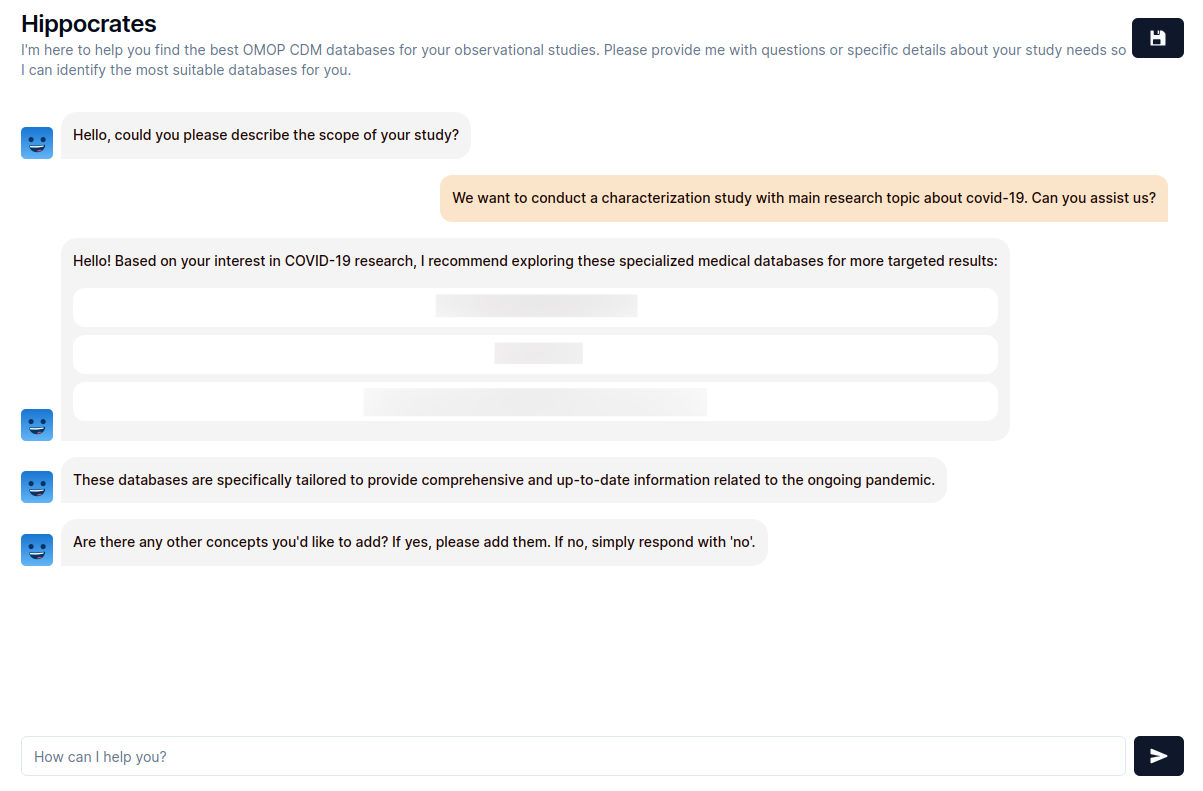
\includegraphics[width=\textwidth]{figs/chapter5/chat1_blur.png}
    \centering
    \caption{Conversation to get the most suitable databases.}
    \label{fig_chat1}
\end{figure}


Therefore, the method of simplifying the discovery of observational databases has an impact on the speed and quality of research efforts. Also, the tool has the potential to level the playing field by providing less experienced individuals with access to complex databases that they might otherwise overlook or find too challenging to navigate. However, the interaction with the proposed tool is somewhat restricted due to the data content. Users may expect to have deep insights into the databases, but that may expose sensitive data. Future enhancements could include the integration of such information available only to users with access to them, which will include the use of Rule-Based Access Control~(RBAC) mechanisms over this tool.



\section{Query Builder}

% em relação  ao query builder, do cohort todo foi apenas definido o seu concept set e a observation window, uma vez que o resto do cohort mostrou ser complexo para o tempo definido para este projeto. Acredito que com mais tempo o cohort seja definido.

% Contudo, o sistema atual mostra que consegue definir um concept set com sucesso e criar um cohort com o respetivo cocnept set e observation window com sucesso também. Com a funionalidade de enviar diretamente para a instância do ATLAS, estes avanços mostram ser promissores na eficacia e no time-saving.

The Query Builder component of the system is an essential part developed to simplify the process of making cohort definitions on ATLAS platform. The present version allows users to specify concept sets and observation windows for a cohort. Concept set, on the other hand, is what defines study group's overall health outcomes such as relevant medical conditions, procedures and medications while observation window means time frame in which patients' data will be observed. The following figures, Figure \ref{fig_chat2} and Figure \ref{fig_chat3}, shows the continuation of the conversation in Figure \ref{fig_chat1}, where the concept set and cohort are defined, respectively.

\begin{figure}[H]
    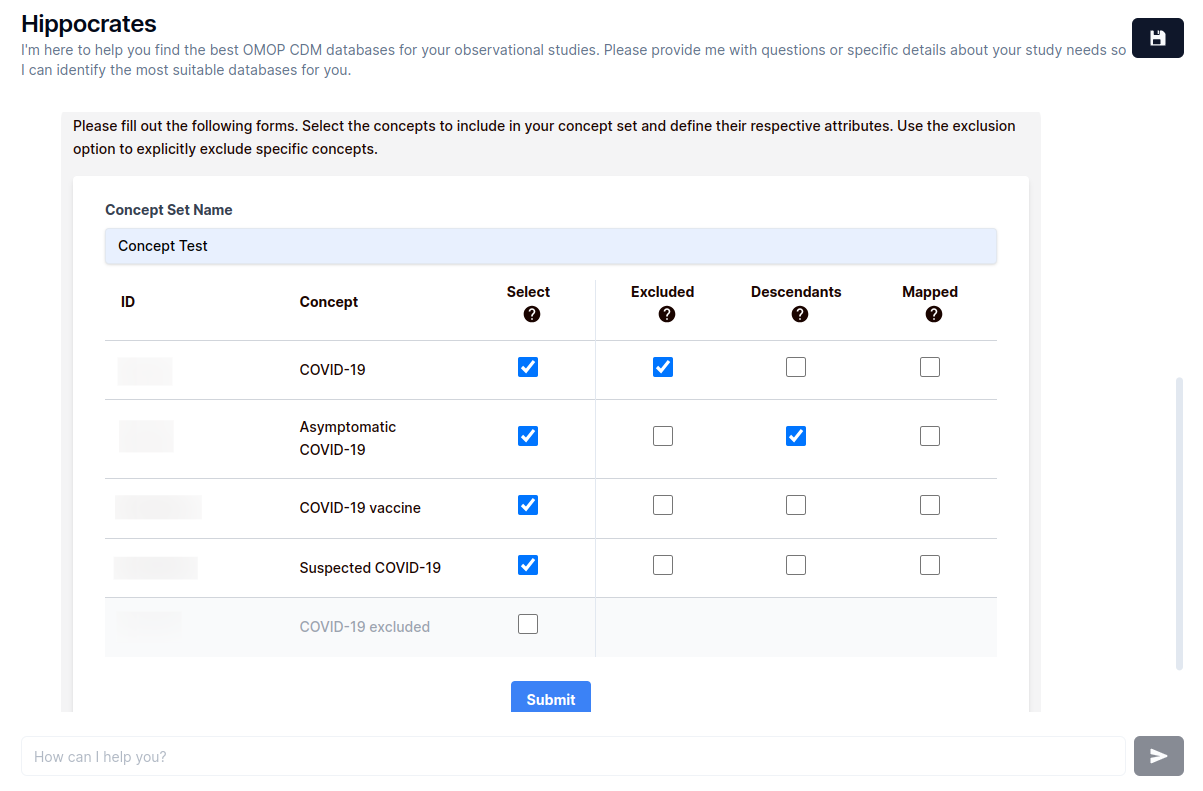
\includegraphics[width=\textwidth]{figs/chapter5/chat2_blur.png}
    \centering
    \caption{Continuing the conversation to define the Concept Set.}
    \label{fig_chat2}
\end{figure}

\begin{figure}[H]
    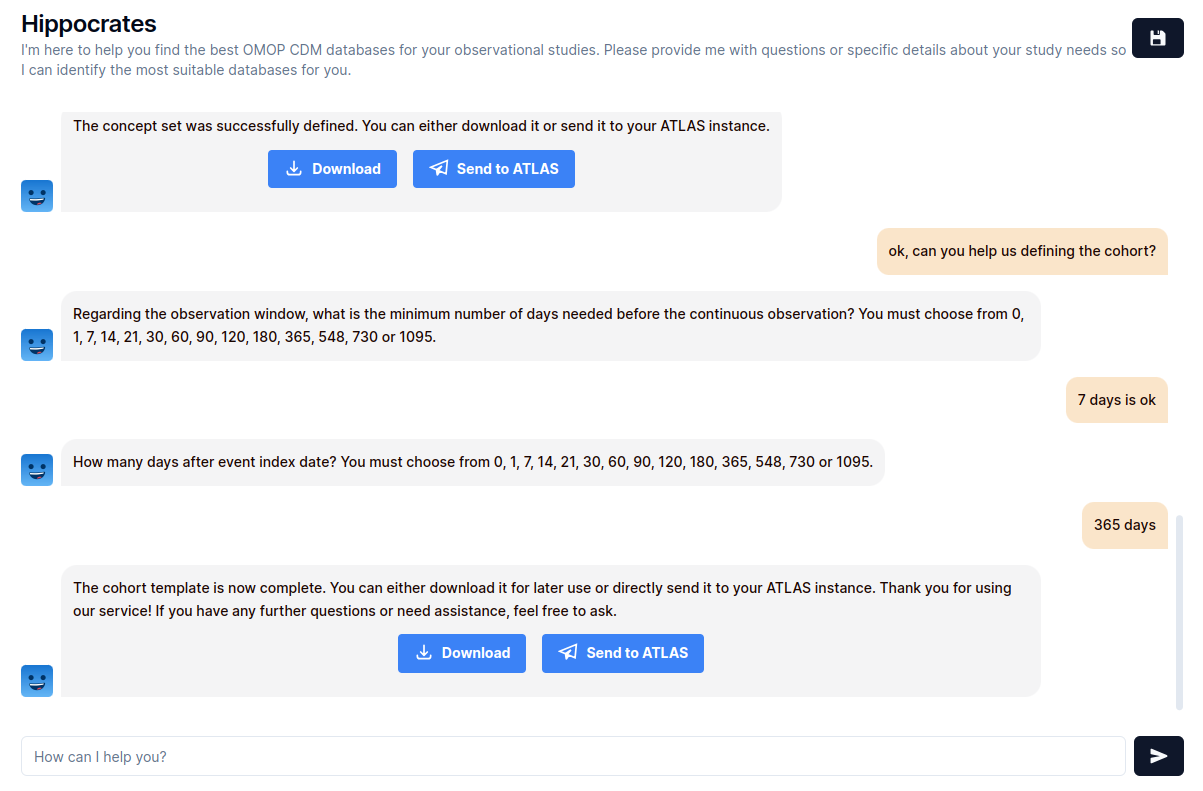
\includegraphics[width=\textwidth]{figs/chapter5/chat3.png}
    \centering
    \caption{Continuing the conversation to define the cohort.}
    \label{fig_chat3}
\end{figure}


One of the significant developments made on the Query Builder is its ability to send defined cohort directly to an instance of ATLAS platform. Being able to send these definitions directly to the ATLAS instance points out considerable improvements towards efficiency as well as time-saving for medical researchers. This shortcut process enhances research quality, reduces errors, and accelerates its pace, facilitating data manipulation for medical researchers dealing with complex observational data.

However, these advancements still face some difficulties. Full cohort definition procedure includes additional parameters like inclusion/exclusion criteria, cohort exit criteria, and cohort attributes that were not fully covered so as not to surpass project's timeline. Some improvements would center on integrating these attributes, enabling the system to better assist researchers in defining their cohorts in their entirety.
